% Circle figure: diameter AB with perpendicular chord CD at E, EF perpendicular to DB at F.
% No extra TikZ libraries required beyond wrapper.
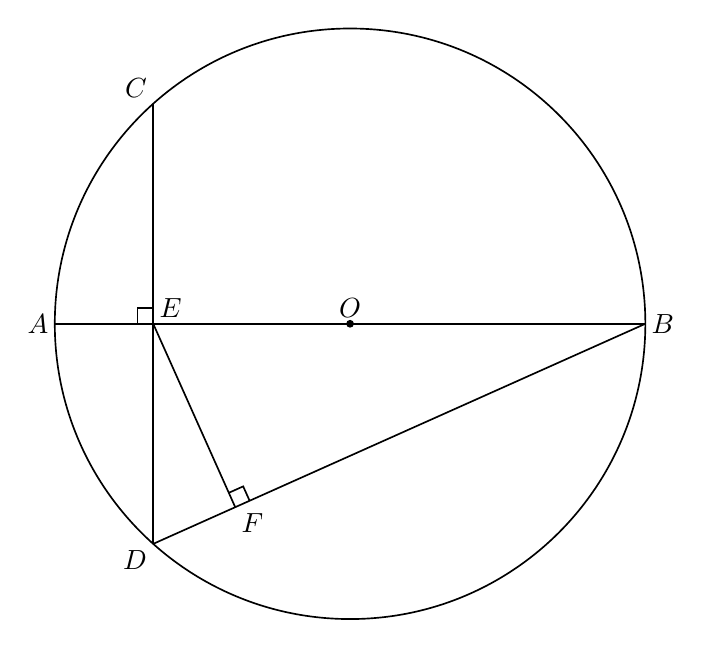
\begin{tikzpicture}[x=1cm,y=1cm,line width=.6pt,font=\normalsize]
\coordinate (O) at (3.75,0.0);
\coordinate (A) at (0.0,0.0);
\coordinate (B) at (7.5,0.0);
\coordinate (E) at (1.25,0.0);
\coordinate (C) at (1.25,2.795085);
\coordinate (D) at (1.25,-2.795085);
\coordinate (F) at (2.291667,-2.329237);
\draw (O) circle [radius=3.75cm];
\draw (A)--(B);
\draw (C)--(D);
\draw (D)--(B);
\draw (E)--(F);
\draw (1.05,0.0)--(1.05,0.20)--(1.25,0.20);
\draw (2.474241,-2.247588)--(2.392591,-2.065014)--(2.210017,-2.146663);
\fill (O) circle [radius=1.4pt];
\node[left=2pt,inner sep=0pt] at (A) {$A$};
\node[right=2pt,inner sep=0pt] at (B) {$B$};
\node[above left=2pt,inner sep=0pt] at (C) {$C$};
\node[below left=2pt,inner sep=0pt] at (D) {$D$};
\node[above right=2pt,inner sep=0pt] at (E) {$E$};
\node[above=2pt,inner sep=0pt] at (O) {$O$};
\node[below right=2pt,inner sep=0pt] at (F) {$F$};
\end{tikzpicture}
